\documentclass[
	letterpaper, % Paper size, specify a4paper (A4) or letterpaper (US letter)
	10pt, % Default font size, specify 10pt, 11pt or 12pt
]{CSUniSchoolLabReport}

%----------------------------------------------------------------------------------------
%	REPORT INFORMATION
%----------------------------------------------------------------------------------------

\title{Lab One\\ Power Systems Analysis \\ EECE5682} % Report title

\author{Michael \textsc{Brodskiy}\\ \small \href{mailto:Brodskiy.M@Northeastern.edu}{Brodskiy.M@Northeastern.edu}}

\date{September 26, 2024} % Date of the report

%----------------------------------------------------------------------------------------


\begin{document}

\maketitle % Insert the title, author and date using the information specified above

\begin{center}
	\begin{tabular}{l r}
		Date Performed: & \today \\ % Date the experiment was performed
		Instructor: & Professor \textsc{Abur} \\ % Instructor/supervisor
	\end{tabular}
\end{center}

\newpage

\begin{abstract}

  This laboratory experiment explores three-phase circuit modeling via SimuLink integration into MATLAB. The experiment simulates a provided circuit design and demonstrates the differences in output power of balanced and unbalanced three-phase conditions.

\end{abstract}

\begin{flushleft}

  \textsc{Keywords:} \underline{three-phase}, \underline{modeling}, \underline{SimuLink}, \underline{MATLAB}, \underline{power}, \underline{balanced}, \underline{unbalanced}

\end{flushleft}

\newpage

\section{Introduction \& Objectives}

This experiment begins by integrating the following diagram into MATLAB's SimuLink environment:

\begin{figure}[H]
  \centering
  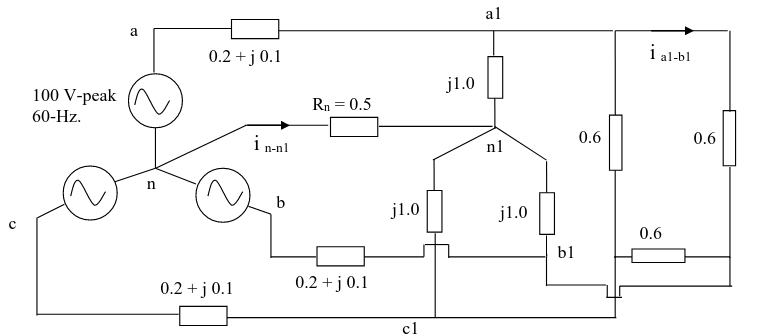
\includegraphics[width=\textwidth]{Figures/Lab\ One/Diagram.png}
  \caption{Simulated Circuit}
  \label{fig:1}
\end{figure}

After simulating the circuit, data related to the instantaneous power, voltage, and current, is taken to calculate expected values. The experiment is then repeated for an unbalanced circuit with $R_a=20[\si{\ohm}]$. For the balanced case, we assume $|V_{in}|=1[\si{\volt}]$, with phase angles $0^{\circ}, 120^{\circ}$, and $-120^{\circ}$.

\section{Results \& Analysis} 

\subsection{Balanced Case ($R_a=2[\si{\ohm}]$)}

The first step of the experiment is to plot the per-phase instantaneous power versus time:

  \begin{figure}[H]
    \centering
    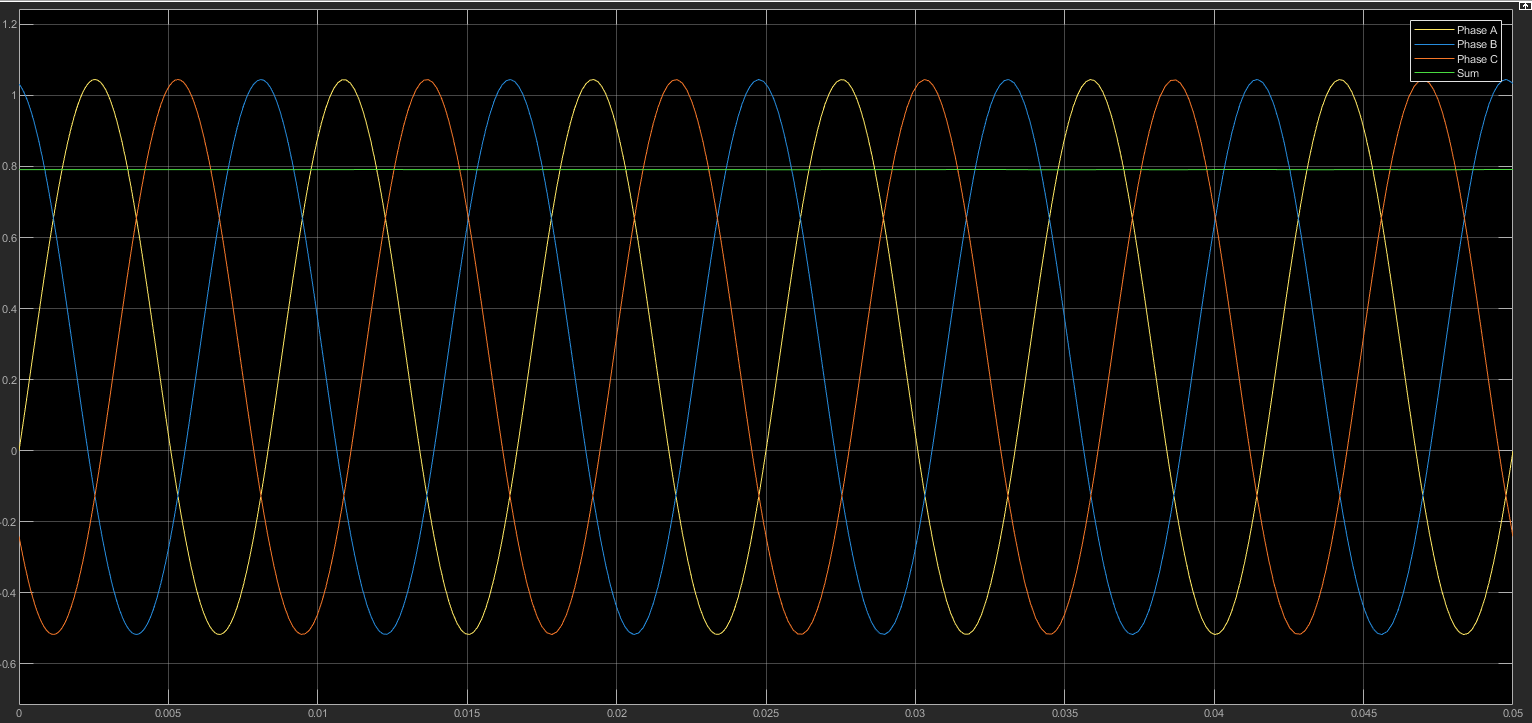
\includegraphics[width=.9\textwidth]{Figures/Lab\ One/InstPower.PNG}
    \caption{Instantaneous Power of the Balanced Circuit Shown in Figure \ref{fig:1}}
    \label{fig:2}
  \end{figure}

  As expected for a balanced circuit, each power is equivalent in magnitude, but with an offset of phase proportional to $120^{\circ}$. From here, we use the Fourier transform blocks to obtain the phasors for $V_{in}$ and $I_{ni}$, respectively. The blocks are shown in Figures \ref{fig:3}-\ref{fig:5} below:

  \begin{multicols}{3}

    \begin{figure}[H]
      \centering
      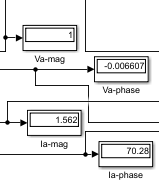
\includegraphics[width=.3\textwidth,height=.2\textheight]{Figures/Lab\ One/VaIa.PNG}
      \caption{Voltage and Current Phasor Blocks, Phase $a$}
      \label{fig:3}
    \end{figure}

    \begin{figure}[H]
      \centering
      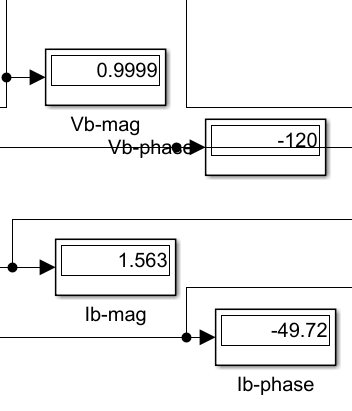
\includegraphics[width=.3\textwidth,height=.2\textheight]{Figures/Lab\ One/VbIb.PNG}
      \caption{Voltage and Current Phasor Blocks, Phase $b$}
      \label{fig:4}
    \end{figure}

    \begin{figure}[H]
      \centering
      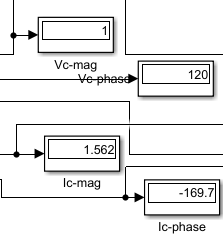
\includegraphics[width=.3\textwidth,height=.2\textheight]{Figures/Lab\ One/VcIc.PNG}
      \caption{Voltage and Current Phasor Blocks, Phase $c$}
      \label{fig:5}
    \end{figure}
  \end{multicols}

  From the blocks, the phasors for voltage and current may be observed as:

  $$\hat{V}_{[a,b,c]n}=1\angle\left[ \begin{matrix} 0\\-120\\120 \end{matrix}\right]^{\circ}[\si{\volt}]$$
  $$\hat{I}_{n[a,b,c]}=1.562\angle\left[ \begin{matrix} 70.28\\-49.72\\-169.72 \end{matrix}\right]^{\circ}[\si{\ampere}]$$

  From here, we may solve for the apparent power using the formula:

  $$\hat{S}=\frac{1}{2}\left[|\hat{V}||\hat{I}|\cos(\phi)+j|\hat{V}||\hat{I}|\sin(\phi)\right]$$

  This gives us:

  $$\hat{S}_{[a,b,c]}=\frac{1}{2}\left[|1||1.562|\cos(-70.28)+j|1||1.562|\sin(-70.28)\right]$$
  $$\hat{S}_{[a,b,c]}=.2635-.7352j[\si{\volt\ampere}]$$

  Thus, we see each source delivers $.2635[\si{\watt}]$ of real power and $-.7352[\text{VAr}]$ of reactive power.\\

  Looking at Figure \ref{fig:2}, we see that the sum power (the green line) is just below $.8[\si{\watt}]$. This makes sense, as, summing the power values of all of the phases gives us a corresponding (DC power) value:

  $$3(.2635)=.7905[\si{\watt}]\approx P_{tot}$$

  The instantaneous three-phase power may be seen in Figure \ref{fig:6} below:

  \begin{figure}[H]
    \centering
    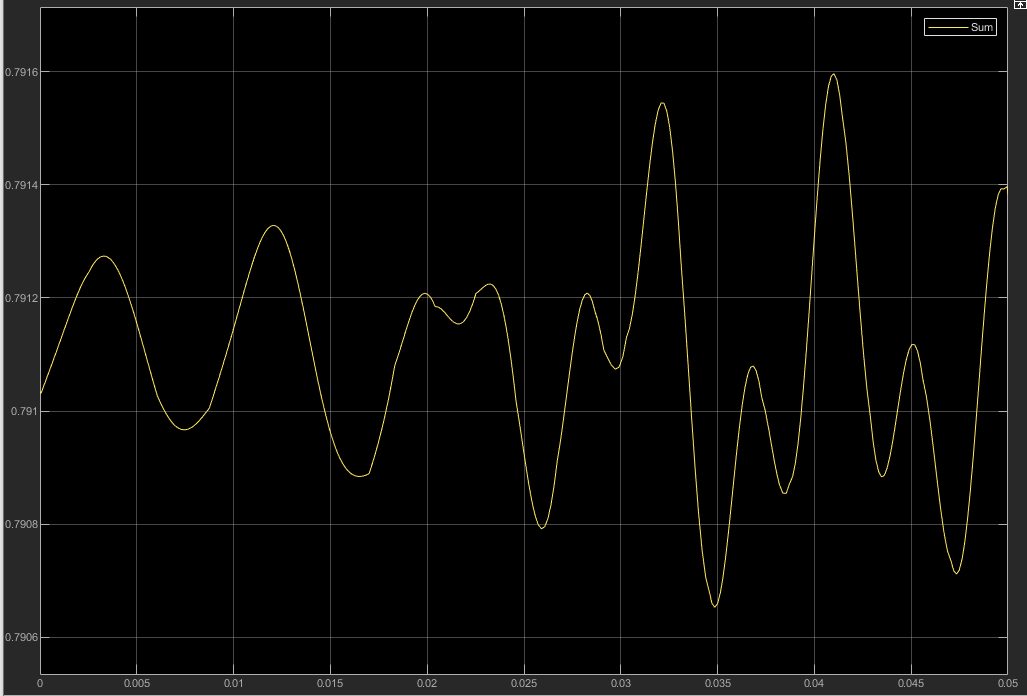
\includegraphics[width=.9\textwidth]{Figures/Lab\ One/Pt.PNG}
    \caption{Instantaneous Power}
    \label{fig:6}
  \end{figure}

  Although it appears that the power fluctuates, further inspection of the waveform shows that it, more or less stays around the expected value of $.7905[\si{\watt}$, with fluctuations of no more than $\pm10^{-2}$, most likely a result of the simulation. Thus, the green line in Figure \ref{fig:1} provides the best approximation, as a balanced three-phase circuit would generate constant instantaneous total power. We now proceed to analyzing an unbalanced circuit.

\subsection{Unbalanced Case ($R_a=20[\si{\ohm}]$)}

The first step of the experiment is to plot the per-phase instantaneous power versus time:

  \begin{figure}[H]
    \centering
    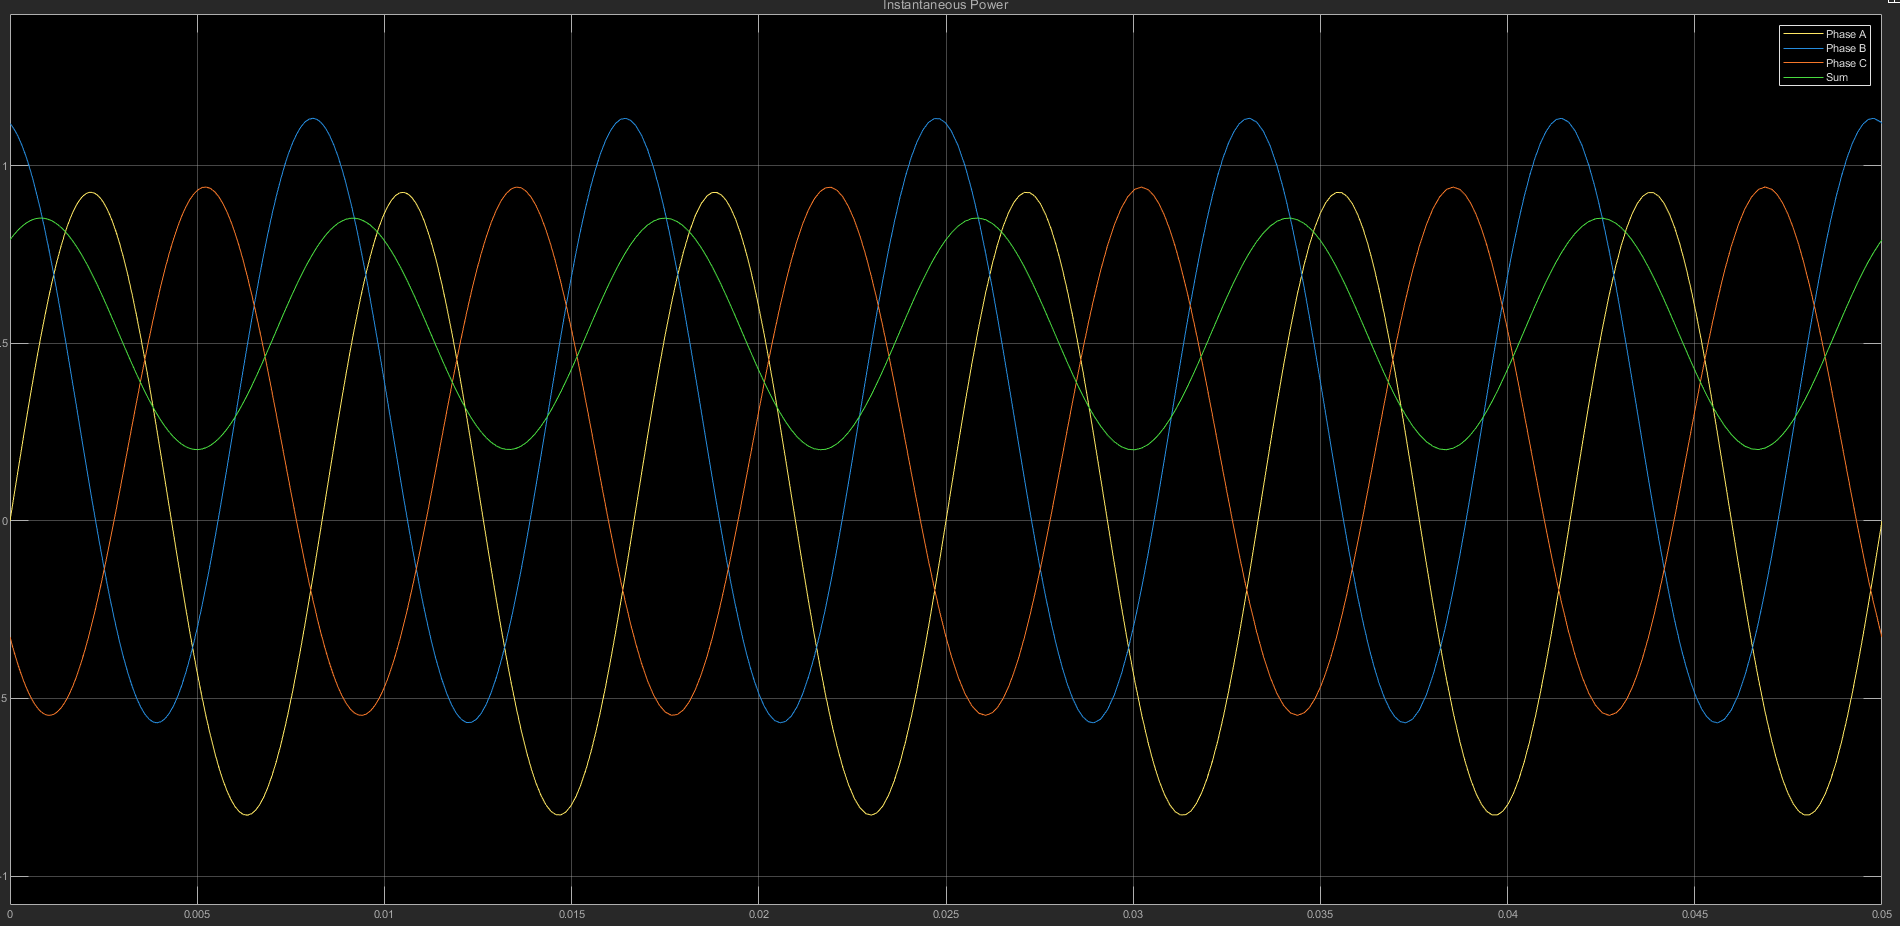
\includegraphics[width=.9\textwidth]{Figures/Lab\ One/InstPower2.PNG}
    \caption{Instantaneous Power of an Unbalanced Circuit Shown in Figure \ref{fig:1}}
    \label{fig:7}
  \end{figure}

  Unlike the balanced case, we see that the powers vary in magnitude, as well as phase. This is expected, as the change of one resistor value would cause a different power delivery in phase $a$, and the same power delivery in phases $b$ and $c$. From here, we use the Fourier transform blocks to obtain the phasors for $V_{in}$ and $I_{ni}$, respectively. The blocks are shown in Figures \ref{fig:8}-\ref{fig:10} below:

  \begin{multicols}{3}

    \begin{figure}[H]
      \centering
      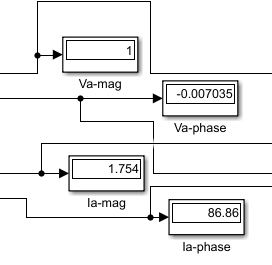
\includegraphics[width=.3\textwidth,height=.2\textheight]{Figures/Lab\ One/VaIa2.PNG}
      \caption{Voltage and Current Phasor Blocks, Phase $a$}
      \label{fig:8}
    \end{figure}

    \begin{figure}[H]
      \centering
      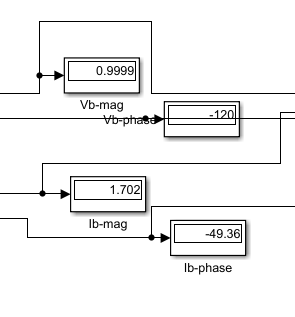
\includegraphics[width=.3\textwidth,height=.2\textheight]{Figures/Lab\ One/VbIb2.PNG}
      \caption{Voltage and Current Phasor Blocks, Phase $b$}
      \label{fig:9}
    \end{figure}

    \begin{figure}[H]
      \centering
      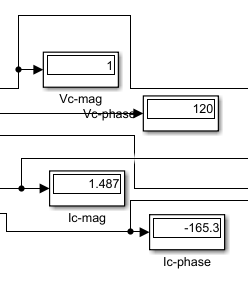
\includegraphics[width=.3\textwidth,height=.2\textheight]{Figures/Lab\ One/VcIc2.PNG}
      \caption{Voltage and Current Phasor Blocks, Phase $c$}
      \label{fig:10}
    \end{figure}
  \end{multicols}

  From the blocks, the phasors for voltage and current may be observed as:

  $$\hat{V}_{[a,b,c]n}=1\angle\left[ \begin{matrix} 0\\-120\\120 \end{matrix}\right]^{\circ}[\si{\volt}]$$
  $$\hat{I}_{n[a,b,c]}=\left[ \begin{matrix}1.754\\1.702\\1.487 \end{matrix} \right]\angle\left[ \begin{matrix} 86.86\\-49.36\\-165.3 \end{matrix}\right]^{\circ}[\si{\ampere}]$$

  We once again solve for the apparent power. This gives us:

  $$\hat{S}_{[a]}=\frac{1}{2}\left[|1||1.754|\cos(-86.86)+j|1||1.754|\sin(-86.86)\right]$$
  $$\hat{S}_{[b]}=\frac{1}{2}\left[|1||1.702|\cos(-70.64)+j|1||1.702|\sin(-70.64)\right]$$
  $$\hat{S}_{[c]}=\frac{1}{2}\left[|1||1.487|\cos(-74.27)+j|1||1.487|\sin(-74.27)\right]$$
  $$\hat{S}_{[a,b,c]}=\left[ \begin{matrix} .048038\\ .2821\\ .1962\end{matrix} \right]+ j\left[ \begin{matrix} -.875683\\-.8029\\-.7171 \end{matrix} \right][\si{\volt\ampere}]$$

  Thus, we see each source delivers a differing amount of real and reactive power, which is to be expected in an unbalanced circuit. The real and reactive powers, respectively, are shown below:

  $$P=\left[ \begin{matrix} .048038\\ .2821\\ .1962\end{matrix} \right][\si{\watt}]\quad\text{ and }\quad Q=\left[ \begin{matrix} -.875683\\-.8029\\-.7171 \end{matrix} \right][\text{VAr}]$$

  Looking at Figure \ref{fig:7}, we see that the sum power (the green line), due to the unbalanced conditions, generates a sinusoid. We may also see that the sinusoid is, on average, just above $.5[\si{\watt}]$. Once again, if we sum these powers, we find the average total power (DC power):

  $$.048038+.2821+.1962=.5263[\si{\watt}]\approx P_{avg}$$

  The instantaneous three-phase power may be seen in Figure \ref{fig:6} below:

  \begin{figure}[H]
    \centering
    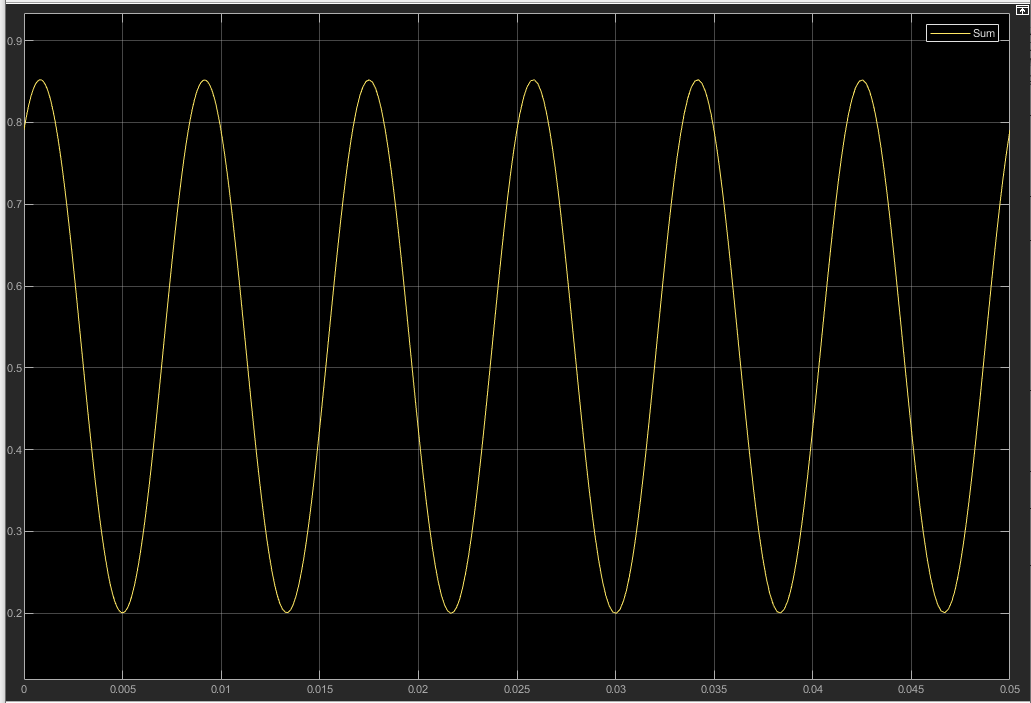
\includegraphics[width=.9\textwidth]{Figures/Lab\ One/Pt2.PNG}
    \caption{Instantaneous Power}
    \label{fig:6}
  \end{figure}

  As expected, we see that the instantaneous power of an unbalanced three-phase circuit behaves in a manner similar to a single phase circuit (that is, it forms a sinusoid with frequency twice that of the voltage/current).

\section{Conclusion}

\begin{enumerate}

  \item With the balanced circuit, the frequency of each phase's power doubles (that is, it goes from the $60[\si{\hertz}]$ of the voltage and current to $120[\si{\hertz}]$). The derivation for the instantaneous power may be found below:

    In a given circuit, assume the voltage and current take the form: $v(t)=V_{max}\cos(\omega t+\theta_v)$ and $i(t)=I_{max}\cos(\omega t+\theta_i)$. The instantaneous power is then:

    $$p(t)=V_{max}I_{max}\cos(\omega t+\theta_v)\cos(\omega t+\theta_i)$$

    Using trigonometric identities and $\phi=\theta_v-\theta_i$, we may write:

    $$p(t)=V_{max}I_{max}[\cos(\phi)+\cos(2\omega t+\theta_v +\theta_i)]$$

    Eliminating the average power (DC offset), we see:

    $$\boxed{p(t)-p_{avg}=V_{max}I_{max}\cos(2\omega t+\theta_v +\theta_i)}$$

    Note that in the sinusoid, ignoring the phase offset, the frequency is doubled ($\omega\to 2\omega$). For this reason, the power experiences $120[\si{\hertz}]$ instead of $60[\si{\hertz}]$.

  \item For a balanced circuit, the frequency of the instantaneous power is $0[\si{\hertz}]$, as the power should not fluctuate I\textit{i}.\textit{e}. it is constant). For the unbalanced circuit, the frequency is twice that of the voltage/current.

\end{enumerate}

\end{document}
